% !TEX root = ../main.tex
% =====================================================================
% 8. RESULTS
%
% Every number here comes from a file, never from my hand:
%   results/SEA_NET/leaderboard.csv          (one row per model)
%   results/SEA_NET/<model>/results.csv      (one row per dataset per seed)
%   results/SEA_NET/profile.csv              (FLOPs, latency, memory)
% Rebuild them all with: python main.py leaderboard && python main.py paper
% =====================================================================

\section{Results}
\label{sec:results}

I compare 72 model variants: my \seanet{} encoders paired with my pooling heads and with
\millet{}'s heads, plus the FCN, ResNet and InceptionTime baselines I re-trained myself. Every model
is run on \webtraffic{} and on the \ucr{} archive, so up to 129 datasets per model.

Two rules hold everywhere, so I state them once. First, my four main models were trained with
\textbf{3 seeds} and show a real mean $\pm$ standard deviation; the rest of the sweep is seed~0
only, because 72 variants over 129 datasets was already close to my compute budget
(\Cref{sec:setup:protocol}). Second, a number I produced is never mixed in the same column with a
number copied from \citet{early2024millet}, because the two use different recipes.

% ---------------------------------------------------------------------
\subsection{Main comparison on \webtraffic{}}
\label{sec:res:web}

\webtraffic{} is the only dataset where I can check both things at once: is the prediction right,
and is the explanation pointing at the real evidence?

\begin{table}[t]
\caption{\webtraffic{} results. The first four rows are the mean $\pm$ standard deviation over
3 seeds; ResNet and FCN have one seed only. Higher is better for accuracy, AOPCR and NDCG@$n$;
lower is better for parameters. AOPCR is not normalised (\Cref{sec:bg:metrics}), so its values are
comparable between these rows only, never with a number printed in another paper.}
\label{tab:web_main}
\begin{center}
\small
\begin{tabular}{lcccr}
\toprule
\textbf{Model} & \textbf{Accuracy} & \textbf{AOPCR} & \textbf{NDCG@$n$} &
\textbf{Params} \\
\midrule
\multicolumn{5}{l}{\emph{Proposed (mine)}}\\
\texttt{seanet\_gated\_mean\_topk}    & $\mathbf{0.955}\pm0.003$ & $2.225\pm0.131$ & $0.750\pm0.022$ & 61{,}740 \\
\texttt{seanet\_bottleneck\_topk}     & $0.947\pm0.016$ & $2.621\pm0.214$ & $\mathbf{0.773}\pm0.013$ & \textbf{41{,}324} \\
\texttt{seanet\_inputgate\_adaptive}  & $0.905\pm0.030$ & $\mathbf{2.651}\pm0.437$ & $0.732\pm0.043$ & 58{,}102 \\
\midrule
\multicolumn{5}{l}{\emph{Baselines re-trained by me, same recipe}}\\
\millet{} (InceptionTime + Conjunctive) & $0.887\pm0.010$ & $2.569\pm0.884$ & $0.677\pm0.016$ & 423{,}707 \\
ResNet + Conjunctive                    & 0.772 & 2.952 & 0.554 & 506{,}331 \\
FCN + Conjunctive                       & 0.742 & 3.826 & 0.533 & 267{,}035 \\
\bottomrule
\end{tabular}
\end{center}
\end{table}
% Source: the WebTraffic rows of each model's results.csv (seeds 0/1/2), mean and sample std
% (ddof=1). These match the web_acc / web_aopcr / web_ndcg columns of leaderboard.csv, which is the
% same seed-average computed by the pipeline.
% NOTE on the published MILLET number: leaderboard.csv's millet_acc (0.8445) is the published UCR-85
% mean, NOT a WebTraffic number -- comparison_vs_millet.csv has no "WebTraffic" row at all. So it
% belongs in the UCR table, not here.

All three of my models beat all three re-trained baselines on all three metrics at the same time,
with 7 to 10 times fewer parameters. That is the main message. The second message is that the winner
is not the same model for every metric: \texttt{seanet\_gated\_mean\_topk} has the best accuracy
(0.955) and is the most stable of the sweep (std 0.003), while \texttt{seanet\_bottleneck\_topk} is
slightly behind on accuracy (0.947) but wins NDCG@$n$ (0.773) at the smallest size (41{,}324
parameters). So the best classifier and the best explanation-per-cost are two different models.
\texttt{seanet\_inputgate\_adaptive} has the highest mean AOPCR (2.651), but I do not read that as a
win: its lead over \texttt{seanet\_bottleneck\_topk} (2.621) is much smaller than its own standard
deviation (0.437), and it is the noisiest model here (accuracy 0.880--0.938 across seeds, against
0.938--0.966).

Nothing was traded away for the better explanation. \texttt{seanet\_bottleneck\_topk} has both the
best NDCG@$n$ and the second-best accuracy, which is what Top-$k$ pooling was designed to do
(\Cref{sec:pool:topk}): it averages only the $k$ most decisive time steps, so the interpretation is
literally zero everywhere the model did not use as evidence, instead of a small non-zero weight
spread over the whole series. \Cref{fig:teaser} shows what that looks like on one series: the
baseline's importance curve is never exactly zero, so a reader has to guess where the evidence
stops, while \seanet{}'s is zero almost everywhere and tall in a few places.

\begin{figure}[t]
  \centering
  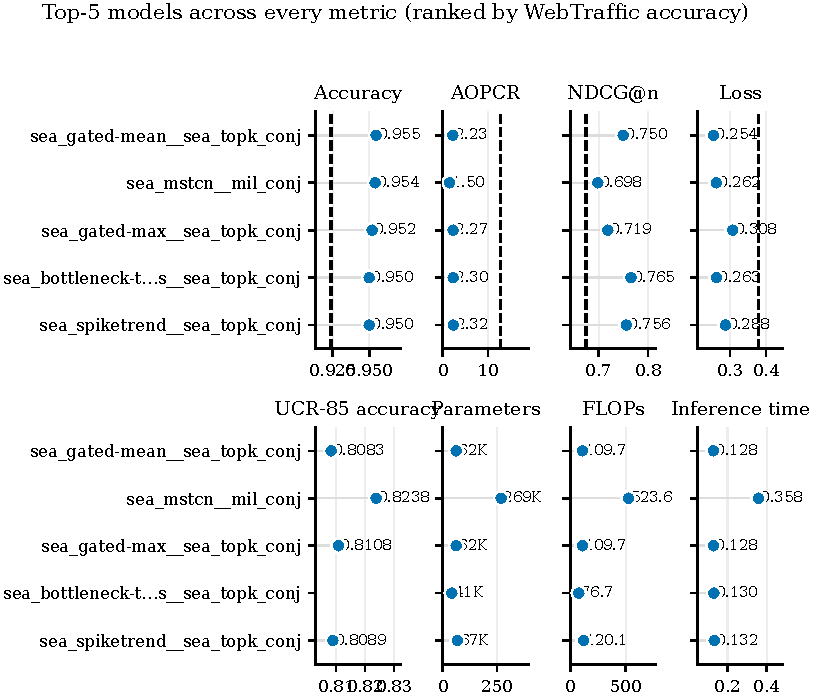
\includegraphics[width=0.85\linewidth]{results/paper_figures/01_main_figures/topk5_multimetric}
  \caption{The five best models by \webtraffic{} accuracy, compared on every metric I measure.
  All panels keep the same model order, so one model can be followed from quality (accuracy,
  AOPCR, NDCG@$n$, loss) across to cost (parameters, FLOPs, latency). Blue marks the models I
  propose in this work. The point of the figure is that the leftmost bars in the quality panels
  are also among the shortest bars in the cost panels.}
  \label{fig:web_bars}
\end{figure}

% ---------------------------------------------------------------------
\subsection{Accuracy across the 85 \ucr{} datasets}
\label{sec:res:ucr}

One dataset proves nothing, so the next question is whether the result holds on the 85 \ucr{}
datasets \millet{} published. I report the mean accuracy, the mean rank and the win/tie/loss record
per dataset, because a mean can hide a model that wins hugely on three datasets and loses
everywhere else.

\begin{table}[t]
\caption{Accuracy over the \ucr{} datasets published by \millet{}. ``Mean rank'' is the average
accuracy rank over 84 datasets among the 27 models with a complete sweep (lower is better).
``W/T/L'' is the win / tie / loss record per dataset against the \emph{published} \millet{}
numbers, where a tie means the two accuracies are within 0.005.}
\label{tab:ucr_accuracy}
\begin{center}
\footnotesize
\begin{tabular}{lccc}
\toprule
\textbf{Model} & \textbf{Mean accuracy} & \textbf{Mean rank} &
\textbf{W/T/L vs published} \\
\midrule
\texttt{seanet\_gated\_mean\_topk}   & 0.8083 & 14.58 & 18 / 13 / 53 \\
\texttt{seanet\_bottleneck\_topk}    & 0.8097 & 14.71 & 19 / 15 / 50 \\
\texttt{seanet\_inputgate\_adaptive} & 0.8153 & 14.79 & 19 / 15 / 50 \\
\millet{} re-trained by me   & \textbf{0.8274} & \textbf{11.86} & 13 / 25 / 46 \\
ResNet + Conjunctive         & 0.8146 & 12.89 & 25 / 11 / 48 \\
FCN + Conjunctive            & 0.8141 & 13.82 & 20 / 12 / 52 \\
\midrule
\millet{} \citep{early2024millet}, published & 0.8445 & -- & -- \\
\bottomrule
\end{tabular}
\end{center}
\end{table}
% Mean accuracy: leaderboard.csv, ucr85_acc column (already averaged over the 85 datasets and over
% every seed the model has). Mean rank + W/T/L: results/paper_figures/tables/table_ranking_accuracy.csv,
% regenerated 2026-08-10 -- computed over the 84 datasets every fully-swept model shares.
% The published row: millet_acc = 0.8445 from leaderboard.csv. Mean rank and W/T/L are left blank
% because the published per-dataset numbers needed to compute them were never carried through -
% only the mean. Do not average this row with the "re-trained by me" row: different recipes.

This table tells a different story from \Cref{tab:web_main}, and I want to say it plainly instead of
hiding it. Over the 85 \ucr{} datasets my re-trained \millet{} baseline is the best of the six: the
highest mean accuracy (0.8274) and the best mean rank (11.86). All three of my models sit around
rank 14.6--14.8 and lose more datasets than they win. I do not think this cancels the \webtraffic{}
result, but it shows its limit: both headline models were chosen because they did well on
\webtraffic{} (\Cref{sec:setup:data}), and one dataset cannot predict what happens on 85 very
different ones. \seanet{} is still competitive -- within 1 to 2 accuracy points of the baseline at
about a tenth of the parameters -- but ``better everywhere'' is a claim this table does not support.
Against the published number (0.8445) my re-trained baseline lands slightly lower (0.8274), which is
the size of gap a different recipe can easily produce (\Cref{sec:disc:reading}).
\missing{\texttt{sv1/millet\_paper} was still sweeping \ucr{} when this was written. When it
finishes (check \texttt{ucr85\_n} = 85 in \texttt{leaderboard.csv}), re-run
\texttt{python main.py leaderboard / results / report / paper} and add its \ucr{} row here --
that is the number that closes objective O2.}

\begin{figure}[t]
  \centering
  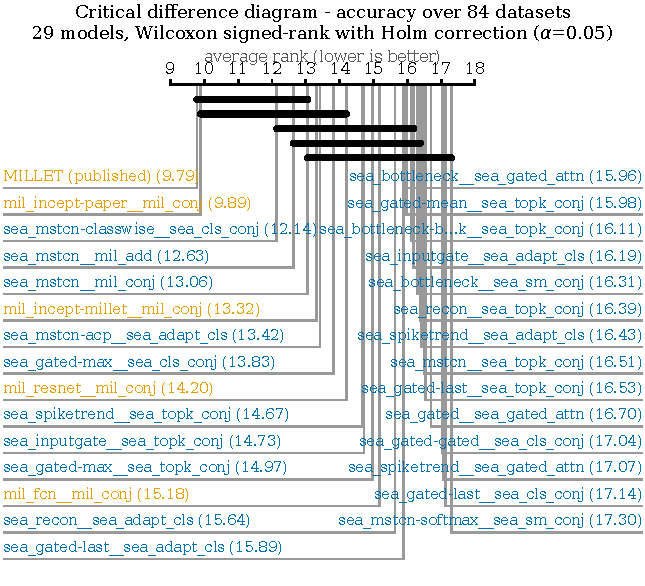
\includegraphics[width=0.85\linewidth]{results/paper_figures/01_main_figures/fig4_critical_difference_accuracy}
  \caption{Critical difference diagram over 84 \ucr{} datasets for the 27 models with a complete
  sweep \citep{demsar2006statistical}. Each model sits on the axis at its average accuracy rank, the
  best on the left. A thick bar joins models whose differences are too small to be trusted (Wilcoxon
  signed-rank test with Holm correction, $\alpha = 0.05$), so two models on the same bar should be
  read as ``I cannot tell them apart''.}
  \label{fig:cd}
\end{figure}

% ---------------------------------------------------------------------
\subsection{Model cost}
\label{sec:res:cost}

Goal~G1 of \Cref{sec:arch:goals} was ``smaller''. This is where I check it, size and speed together,
because a model that is small but slow would not be a real win.

\begin{table}[t]
\caption{Cost of each model, measured at the real \webtraffic{} shape (length 1008, 10 classes,
batch 32) on one GPU. Training time is the wall-clock time to converge including early stopping,
mean $\pm$ standard deviation over the 3 \webtraffic{} seeds.}
\label{tab:cost}
\begin{center}
\small
\begin{tabular}{lrrrrr}
\toprule
\textbf{Model} & \textbf{Params} & \textbf{Size (MB)} & \textbf{FLOPs (M)} &
\textbf{Inference (ms)} & \textbf{Train time (s)} \\
\midrule
\texttt{seanet\_bottleneck\_topk}     & \textbf{41{,}324}  & \textbf{1.43} & \textbf{76.7}  & 0.131 & $117.3\pm14.0$ \\
\texttt{seanet\_inputgate\_adaptive}  & 58{,}102  & 1.49 & 110.6 & 0.128 & $105.8\pm37.2$ \\
\texttt{seanet\_gated\_mean\_topk}    & 61{,}740  & 1.50 & 109.7 & 0.128 & $91.3\pm25.9$ \\
\millet{} re-trained by me            & 423{,}707 & 4.11 & 847.6 & 0.203 & $50.4\pm9.5$ \\
ResNet + Conjunctive                  & 506{,}331 & 4.42 & 1013.2 & 0.139 & 38.1 \\
FCN + Conjunctive                     & 267{,}035 & 3.47 & 535.2 & \textbf{0.068} & 20.8 \\
\bottomrule
\end{tabular}
\end{center}
\end{table}
% Params / Size / FLOPs / Inference: results/SEA_NET/profile.csv, re-measured 2026-08-09 with
%   python scripts/profile_models.py --length 1008 --classes 10 --batch 32
% Re-profiling at the real WebTraffic shape matters: the earlier profile used a length-500,
% 5-class dummy input, which made the pooling heads look smaller than they are and reported a
% misleading 2.594 ms for seanet_inputgate_adaptive. At the real shape that model is 0.128 ms.
% Train time: the WebTraffic rows of each model's results.csv, mean +- std over seeds 0/1/2.

The parameter cut is large and it is real. \texttt{seanet\_bottleneck\_topk} uses 90\,\% fewer
parameters than the re-trained \millet{} baseline (41{,}324 against 423{,}707), 11$\times$ fewer
FLOPs, and is about 1.6$\times$ faster at inference. All three of my models sit between 1.4 and
1.5\,MB against 4.1\,MB for the baseline, which is the number that matters for a microcontroller
(\Cref{sec:context}).

% ---------------------------------------------------------------------
\subsection{Training behaviour}
\label{sec:res:training}

The last column of \Cref{tab:cost} is the honest counterweight. My models take \emph{longer} to
train than the baseline (roughly 2 to 3 times, on every seed), even though they are 10$\times$
smaller and much cheaper per step. That is not a contradiction: training time here is wall-clock
time until early stopping fires, so it measures how many epochs a model needed, not how expensive
one epoch is. The baseline stops earlier because its validation loss stops improving earlier. FLOPs
and inference time are the honest per-step comparison, and there \seanet{} wins clearly. Whether my
models need more epochs to reach the same loss, or early stopping simply behaves differently for the
two loss shapes, is a question the per-epoch curves can now answer: I changed the code so every run
writes its curve to \texttt{results/SEA\_NET/<model>/curves/}, which was not the case when the main
sweep was run.

% ---------------------------------------------------------------------
\subsection{Ablations}
\label{sec:res:ablation}

The main question is simple: does the gain come from the encoder, from the pooling head, or from
putting the two together? The rest of my ablations, including the top-$k$ fraction and the attention
focus penalty, are in \Cref{app:ablations}.

\begin{figure}[h]
  \centering
  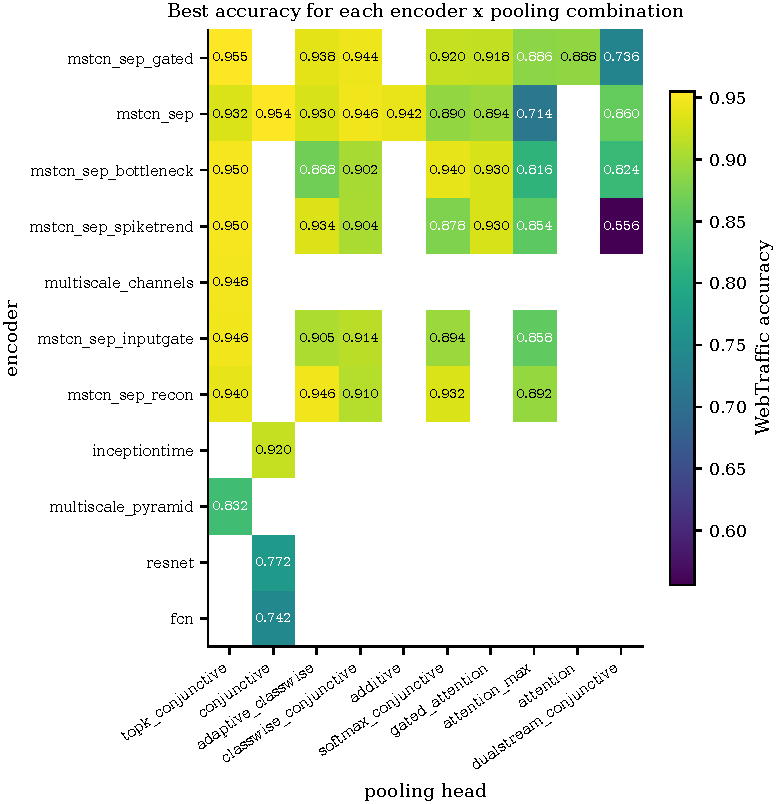
\includegraphics[width=0.85\linewidth]{results/paper_figures/02_ablation/ablation_encoder_pooling_grid}
  \caption{Best \webtraffic{} accuracy for every encoder (rows) and every pooling head (columns).
  Read one cell as ``what this pair achieved''; blank cells are pairs I never trained. Rows and
  columns are sorted by their best value, so the strong components move to the top left.}
  \label{fig:ablation_grid}
\end{figure}

Taken on their own, the encoder and the head matter about equally. Averaged over every head it was
paired with, the encoder moves accuracy from 0.858 (Spike/trend) to 0.937
(\texttt{sea\_multiscale\_channels}); averaged over every encoder, the head moves it from 0.744
(Dual-stream) to 0.921 (Class-wise conjunctive). Two ranges of a similar size, so neither half
dominates. The more interesting result is that the best pair is \emph{not} made of the two best
halves: \texttt{seanet\_gated\_mean\_topk} (0.955) pairs the Gated encoder, which averages 0.902,
with Top-$k$ pooling, which averages 0.904 -- both mid-table. The gain is not the sum of two good
parts, and I could only have found this pair by trying the combination. One caveat to keep visible:
several groups in these averages contain very few models, and not every pair was trained, so the
grid read cell by cell is the more trustworthy view.
